
%(BEGIN_QUESTION)
% Copyright 2004, Tony R. Kuphaldt, released under the Creative Commons Attribution License (v 1.0)
% This means you may do almost anything with this work of mine, so long as you give me proper credit

Write the transfer function (input/output equation) for an operational amplifier with an open-loop voltage gain of 100,000.  In other words, write an equation describing the output voltage of this op-amp ($V_{out}$) for any combination of input voltages ($V_{in(+)}$ and $V_{in(-)}$):

$$\includegraphics[width=15.5cm]{i01471x01.eps}$$

\underbar{file i01471}
%(END_QUESTION)





%(BEGIN_ANSWER)

$V_{out} = 100,000(V_{in(+)} - V_{in(-)})$

%(END_ANSWER)





%(BEGIN_NOTES)

The concept of a ``transfer function'' is very useful, and this may be your students' first exposure to the idea.  It is a phrase used quite often in engineering applications, and may denote an equation, a table of numbers, or a graph.

In this particular question, it is important that students know how to derive and use the basic transfer function for a differential amplifier.  Challenge your students to express this function in a more general form, so that calculations may be made with different open-loop voltage gains.

%INDEX% Electronics review: opamp as a high-gain differential amplifier

%(END_NOTES)


